\documentclass[12pt,reqno]{amsart}
\usepackage{fullpage}
\usepackage{amsfonts}
\usepackage{tikz}
\usepackage{amssymb}
\usepackage{times}
\usepackage{graphicx}
\usepackage{mathtools}
\usepackage{breakurl}
\usepackage{bm}
\usepackage{blkarray}
\usepackage{url}
\usepackage[all]{xy}
\usepackage[margin=0.8in,footskip=0.25in]{geometry}
\usepackage[all]{xy}
\usepackage{tikz}

\usepackage[colorlinks=true,
            linkcolor=red,
            urlcolor=blue,
            citecolor=gray]{hyperref}
\vfuzz=2pt


\DeclarePairedDelimiter\ceil{\lceil}{\rceil}
\DeclarePairedDelimiter\floor{\lfloor}{\rfloor}

\DeclareMathOperator{\cok}{coker}
\DeclareMathOperator{\im}{im}
\DeclareMathOperator{\ann}{Ann}
\DeclareMathOperator{\Hom}{Hom}


% some "funny lines" referred to later:
\newtheorem{theorem}{Theorem}[section]
\newtheorem{corollary}[theorem]{Corollary}
\newtheorem{lemma}[theorem]{Lemma}
\newtheorem{proposition}[theorem]{Proposition}
{\theoremstyle{remark}\newtheorem*{remark}{Remark}}
\theoremstyle{definition}
\newtheorem{definition}[theorem]{Definition}
\newtheorem{example}[theorem]{Example}


\newcommand{\lex}{\mbox{lexdeg}}
\newcommand{\mymod}[3]{#1 \equiv #2 \Mod{#3}}
\newcommand{\ccc}{\mathcal{C}}
\newcommand{\nmm}[2]{\text{N}_{#1}(#2)}
\newcommand{\Mod}[1]{\ (\mathrm{mod}\ #1)}
\newcommand{\gal}{\text{Gal}}
\newcommand{\cc}{\mathbb{C}}
\newcommand{\zz}{\mathbb{Z}}
\newcommand{\ta}[1]{\langle #1 \rangle}
\newcommand{\ff}{\mathbb{F}}
\newcommand{\qq}{\mathbb{Q}}
\newcommand{\Tor}[2]{\mathbf{Tor}_{#1}(#2)}
\newcommand{\sqrtn}[1]{\sqrt[n]{#1}}
\newcommand{\charr}{\text{char}}
\newcommand{\disc}[1]{\mbox{disc}(#1)}
\newcommand{\Aut}{\text{Aut}}
\newcommand{\Inn}{\text{Inn}}
\newcommand{\Gal}{\text{Gal}}
\newcommand{\sgn}{\text{sgn}}
\newcommand{\irr}{\text{irr}}
\newcommand{\of}{\overline{F}}
\newcommand{\ok}{\overline{K}}
\newcommand{\ZZ}{\mathbb{Z}}
\newcommand{\NN}{\mathbb{N}}
\newcommand{\CC}{\mathbb{C}}
\newcommand{\QQ}{\mathbb{Q}}
\newcommand{\RR}{\mathbb{R}}
\newcommand{\FF}{\mathbb{F}}
\newcommand{\Tr}{\text{Tr}}
\newcommand{\nm}{\text{N}}
\newcommand{\tk}{\theta_K}
\newcommand{\mm}{\mathfrak{m}}
\newcommand{\tor}{\mathbf{Tor}}
\newcommand{\conv}[1]{\mathrm{conv}(#1)}
\newcommand{\diam}[1]{\mathrm{diam}(#1)}
\newcommand{\vol}[1]{\mathrm{vol}(#1)}
\newcommand{\la}{\langle}
\newcommand{\ra}{\rangle}

\begin{document}

\title{HW4}

\noindent \textbf{Q1:}

\begin{center}
  \begin{tikzpicture}[scale=3]
    \draw[very thick] (0,0) -- (2,0);
    \draw[very thick] (0,0) -- (1,1.732);
    \draw[very thick] (2,0) -- (1,1.732);
    \draw[very thick] (1,0) -- (1,1.732);
    \draw (0,0) -- (1.5, 0.866);
    \draw (2,0) -- (0.5, 0.866);
    \draw (0.5,0.866) -- (1.5, 0.866);
    \draw[dotted,thick] (0,0) -- (1, 0.866);
    \draw[dotted,thick] (2,0) -- (1, 0.866);
    \draw[dotted,thick] (1,0) -- (0.5, 0.866);
    \draw[dotted,thick] (1,0) -- (1.5, 0.866);
    \filldraw [red] (0,0) circle (1pt);
    \filldraw [red] (1,0) circle (1pt);
    \filldraw [red] (2,0) circle (1pt);
    \filldraw [red] (0.5, 0.866) circle (1pt);
    \filldraw [red] (1, 0.866) circle (1pt);
    \filldraw [red] (1.5, 0.866) circle (1pt);
    \filldraw [red] (1,1.732) circle (1pt);
    \filldraw [red] (1,0.57735) circle (1pt);
  \end{tikzpicture}
\end{center}


As indicated in the figure, the 8 points consist of 3 vertices of an equilateral triangle, 3 midpoints of edges, the mass center and the midpoint of the height. The 4 dotted lines are the ordinary lines.

\newpage
\noindent \textbf{Q2:} We borrow the ideas from graph theory. For each configuration $X$, we associate it with a matrix $m(X)$ with rows labeled by points and columns labeled by lines and with the entry value 1 if the point lies on the line and 0 if not. Relabeling and moving vertices around for a fixed configuration $X$ only permutes rows and columns of $m(X)$. In other words, if $X$ and $Y$ are two isomorphic combinatorial configurations, then there is a permutation matrix $P$ such that $m(Y)=P\cdot m(X)$. In particular, this means $m(X)$ and $m(Y)$ have the same rank.

Now label the Pappus configuration and another configuration as in the figure.

\begin{figure}[h]
  \centering
  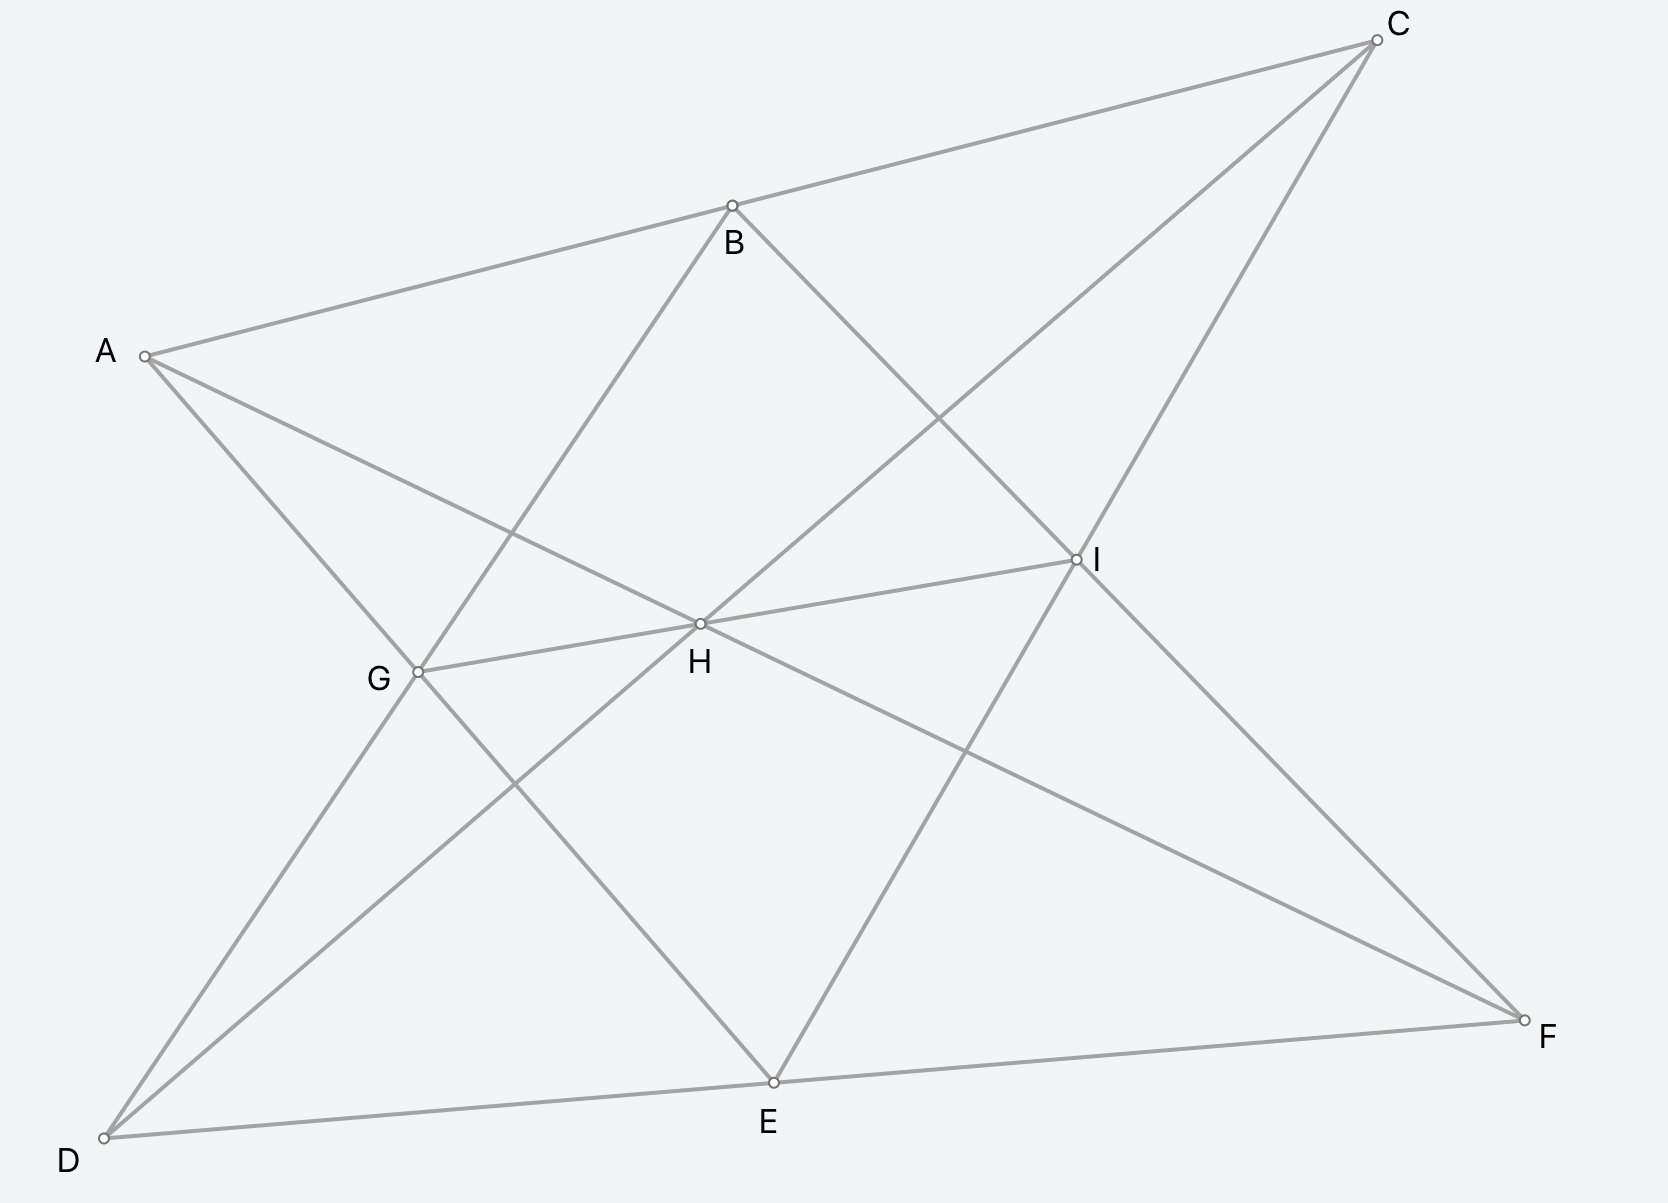
\includegraphics[width=8cm]{hw4a}
  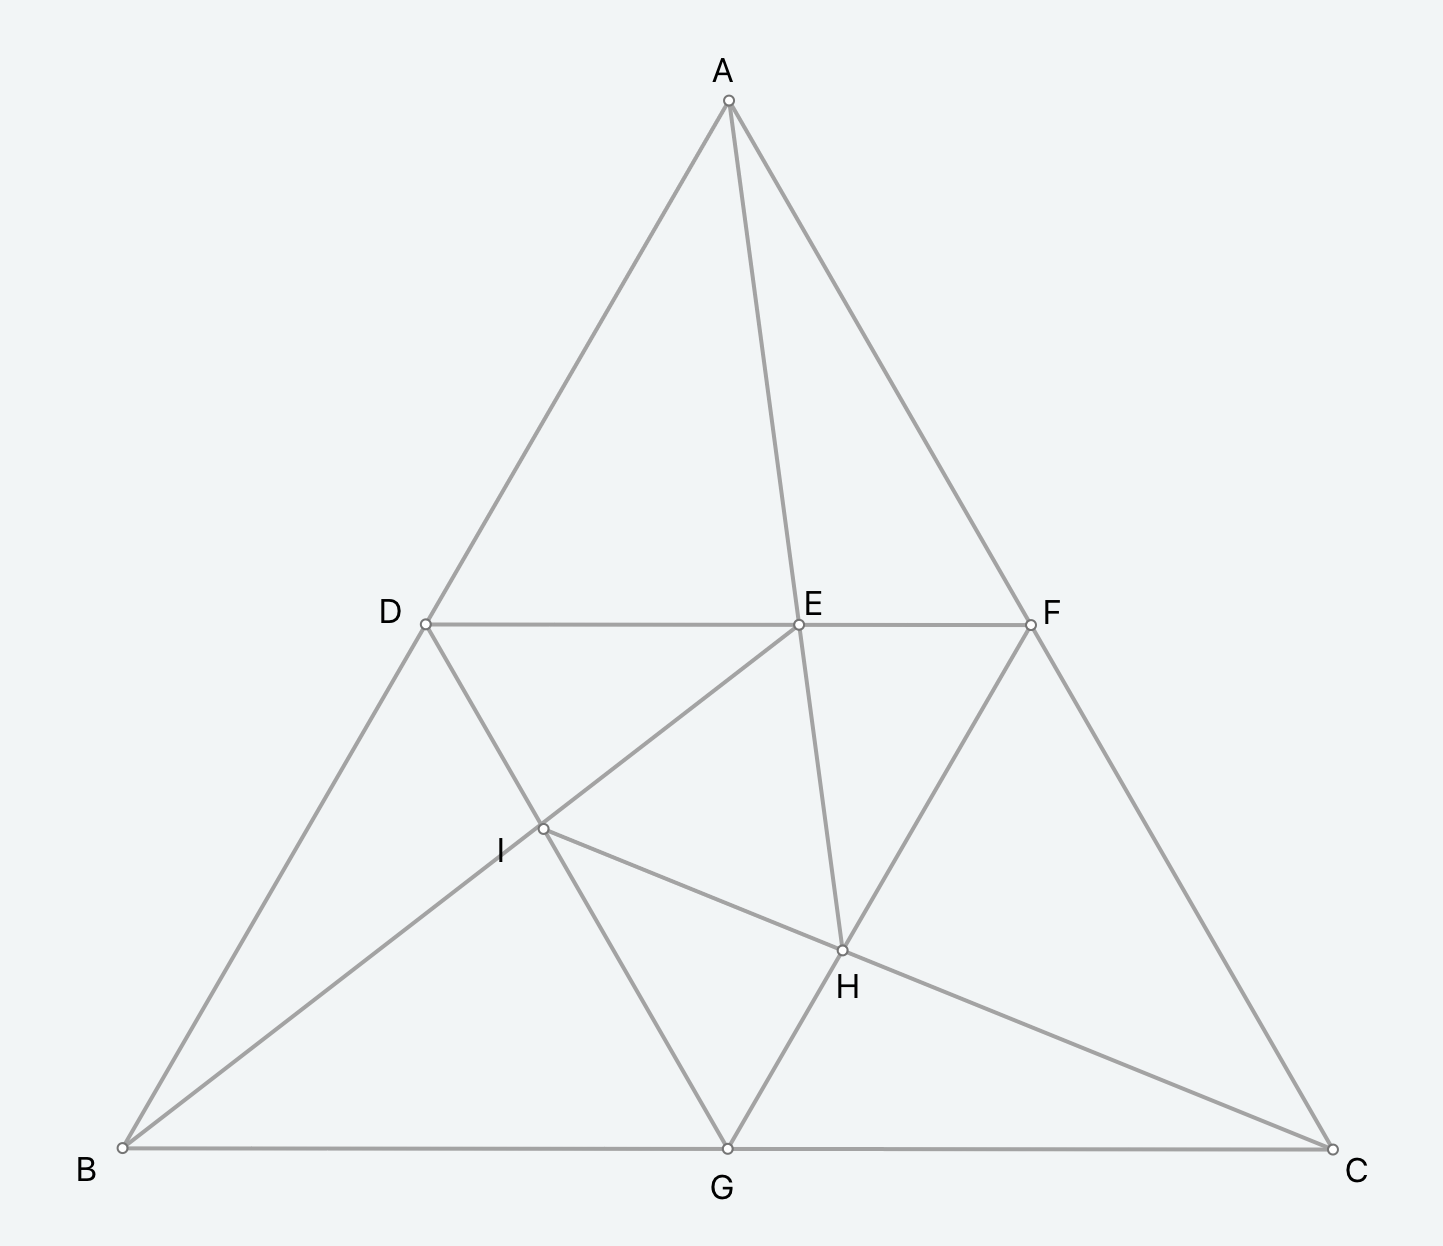
\includegraphics[width=7.5cm]{hw4b}
\end{figure}

Then the associated matrices are
\[
  \begin{blockarray}{cccccccccc}
    & ABC & AHF & AGE & BGD & BIF & CHD & CIE & GHI & DEF \\
    \begin{block}{c(ccccccccc)}
      A & 1 & 1 & 1 & 0 & 0 & 0&0&0&0 \\
      B & 1 & 0 & 0 & 1 & 1&0&0&0&0 \\
      C & 1&0&0&0&0&1&1&0&0\\
      D &0&0&0&1&0&1&0&0&1\\
      E &0&0&1&0&0&0&1&0&1\\
      F &0&1&0&0&1&0&0&0&1\\
      G &0&0&1&1&0&0&0&1&0\\
      H &0&1&0&0&0&1&0&1&0\\
      I &0&0&0&0&1&0&1&1&0\\
    \end{block}
  \end{blockarray} = m(X)
\]
and
\[
  \begin{blockarray}{cccccccccc}
    & ADB & AEH &AFC& BGC&BIE&CHI&DEF&DIG&GHF\\
    \begin{block}{c(ccccccccc)}
      A & 1 & 1 & 1 & 0 & 0 & 0&0&0&0 \\
      B & 1 & 0 & 0 & 1 & 1&0&0&0&0 \\
      C &0&0&1&1&0&1&0&0&0\\
      D &1&0&0&0&0&0&1&1&0\\
      E &0&1&0&0&1&0&1&0&0\\
      F &0&0&1&0&0&0&1&0&1\\
      G &0&0&0&1&0&0&0&1&1\\
      H &0&1&0&0&0&1&0&0&1\\
      I &0&0&0&0&1&1&0&1&0\\
    \end{block}
  \end{blockarray} = m(Y).
\]

But a straightforward calculation gives $\det(m(X)) = 0$ and $\det(m(Y))=27$. It follows that $m(X)$ and $m(Y)$ do not have the same rank and these two configurations are not isomorphic.


\newpage
\noindent \textbf{Q3:}

\begin{center}
  \begin{tikzpicture}[scale=1.5]
    \draw[very thick](0,0) circle (1);
    \draw[very thick](1.73205,0) circle (1);
    \draw[very thick](0.866,0.5) circle (1);
    \draw[very thick](0.866,1.5) circle (1);
    \filldraw [red] (0, 0) circle (1pt);
    \filldraw [red] (1.73205,0) circle (1pt);
    \filldraw [red] (0.866,0.5) circle (1pt);
    \filldraw [red] (0.866,1.5) circle (1pt);
  \end{tikzpicture}
\end{center}

As shown in the figure, the centers of the unit circles are $(0,0),(\sqrt{3},0),(\frac{\sqrt{3}}{2},\frac{1}{2})$ and $(\frac{\sqrt{3}}{2},\frac{3}{2})$.


\newpage
\noindent \textbf{Q4:}


\newpage
\noindent \textbf{Q5:}


\newpage
\noindent \textbf{Q6:}



\newpage
\noindent \textbf{Q7:}

\end{document}


